\documentclass[10pt,fleqn,a4paper]{jsarticle}
\usepackage[dvipdfmx]{graphicx,color}
\usepackage{ascmac,amsmath,amssymb,amstext}
\usepackage{tikz,multicol,float,tikz-3dplot}
\usetikzlibrary{positioning,intersections,calc,arrows.meta,math,angles}
\usepackage{zogeny,ceo,comment}
\newcommand{\ans}[1]{\mbox{\boldmath{$#1$}}}
\renewcommand{\baselinestretch}{1.2} 
\tdplotsetmaincoords{60}{110}%{xy平面からどれだけ上にいるか(90度から-90度)}{z軸中心にどれだけ左右に回転するか}
\begin{document}
\begin{itembox}
[l]{\fbox{\kurosankakub 問題\kurosankakua}}
\kakkoichi  $f(x)=e^{x+1},g(x)=e^{-2x}とするとき,h\p{f(x)}=g(x)なる関数h(x)を求める.\\
\kakkoni  極方程式 r^2-4r\sin\p{\theta+\dfrac{\pi}{3}}+3=0を満たす円の方程式を求める.\\
\kakkosan  \lim_{n\to\infty}\dfrac{1}{n^2}\p{\sqrt{n^2}+\sqrt{n^2-1}+\sqrt{n^2-4}+\cdots+
\sqrt{n^2-(n-1)^2}} を求める.$
\end{itembox}
\kaisetu\\
\kakkoichib  関数の中に関数が入っているのが嫌なので,とりあえず$\ans{f(x)=t}と置いてみることにしました.
そうすると,\\
t=e^{x+1}\doti x=\log\dfrac{t}{e}=\log t-1 となる.これがポイントかなあと.\\
\kakkonib  授業で言った通り,極座標と直交座標系を繋ぐのは,\ans{\tvec<0,1>[x,y]=r\tvec<0,1>[\cos\theta,\sin\theta]}\cdots\asta 
という
関係です.\\これを,少し変形して遊んでみましょう.\\
\asta の両辺を大きさをとって,2乗してみると,$
\begin{align*}
    &\left|\tvec<0,1>[x,y]\right|=r\left|\tvec<0,1>[\cos\theta,\sin\theta]\right|\\
    &\doti \sqrt{x^2+y^2}=r\sqrt{\cos^2\theta+\sin^2\theta}\\
    &\doti \ans{x^2+y^2=r^2} という関係式が導かれます.(\temarku お風呂入っている時に思いつきました\egaob)
\end{align*}
これで,問題で与えられた極方程式を直行座標系の言葉で言い換えることができますね!\\
これは,教科書では「暗記せよ」と書かれていますが,考えれば当たり前ですね.\\

\kakkosanb  授業で言った通り,区分求積法です.定義式は次の通り.
\begin{center}
    $\ans{\lim_{n\to\infty}\wa{k=0}{n-1}\dfrac{1}{n}f\p{\dfrac{k}{n}}
    =\lim_{n\to\infty}\wa{k=1}{n}\dfrac{1}{n}f\p{\dfrac{k}{n}}
    =\dint{0}{1}f(x)dx}$
\end{center}
「なぜ,無限級数の二つの式がイコールになるのか?」という疑問は下の図を見れば分かるはず.
\begin{center}
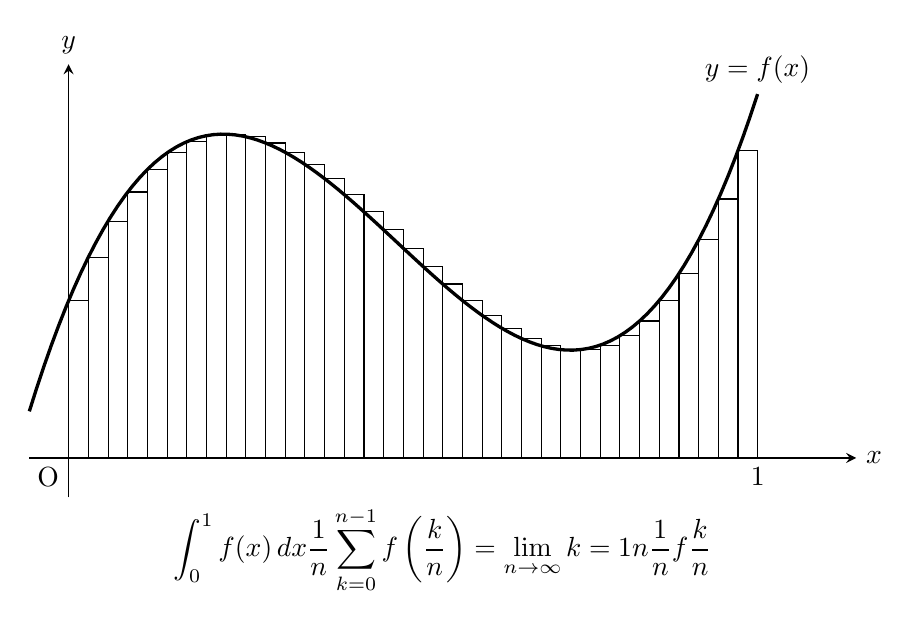
\begin{tikzpicture}[xscale=2.5]
 \coordinate[label=below left:O] (O) at (-2,0); %原点O
 \coordinate(XS)at(-2.2,0); \coordinate(XL)at(2,0); \draw[semithick,->,>=stealth](XS)--(XL)node[right]{$x$}; %x軸
 \coordinate(YS)at(-2,-0.5); \coordinate(YL)at(-2,5); \draw[semithick,->,>=stealth](YS)--(YL)node[above]{$y$}; %y軸
 
 \draw[samples=100,domain=-2.2:1.5,very thick] plot(\x,\x*\x*\x+\x*\x-2*\x+2) node[above] {$y=f(x)$}; %y=f(x)のグラフ
 \foreach \t in {-2,-1.9,...,1.5}
   \draw (\t,0)--(\t,\t*\t*\t+\t*\t-2*\t+2)--(\t+0.1,\t*\t*\t+\t*\t-2*\t+2)--(\t+0.1,0); %x=t,x=t+1の間の短冊
 \draw (1.5,0) node[below]{1}; %点(1,0)
 
 \draw ($(XS)!0.5!(XL)+(0,-0.5)$)
   node[below]{$\displaystyle\int_{0}^{1}f(x)\,dx \yaku\frac{1}{n}\sum_{k=0}^{n-1}f\left(\frac{k}{n}\right)=\lim_{n\to\infty}\wa{k=1}{n}\dfrac{1}{n}f\p{\dfrac{k}{n}}$};
   %図のx軸の中点+(0,-1)の位置に区分求積の式
\end{tikzpicture}
\end{center}
つまり,長方形の縦の長さを左と右のどちらで始めるかによって$「\wa{}{} のスタート」$が変わるということです.\\
分からなかったら鈴木先生に聞いてみてください.(心先生,よろしくお願いします.\hiraayamari)\\
従って,次のような変形をすれば区分求積の形に持っていくことができます.
\begin{align*}
&\dfrac{1}{n^2}\p{\sqrt{n^2}+\sqrt{n^2-1}+\sqrt{n^2-4}+\cdots+\sqrt{n^2-(n-1)^2}}\\
&=\dfrac{1}{n}\p{\dfrac{\sqrt{n^2}}{n}+\dfrac{\sqrt{n^2-1}}{n}+\dfrac{\sqrt{n^2-4}}{n}+\cdots+
\dfrac{\sqrt{n^2-\p{n-1}^2}}{n}}\\
&=\dfrac{1}{n}\p{1+\sqrt{1-\p{\dfrac{1}{n}}^2}+\sqrt{1-\p{\dfrac{2}{n}}^2}+\cdots+\sqrt{1-\p{\dfrac{n-1}{n}}^2}}\\
&=\dfrac{1}{n}\p{\sqrt{1-\p{\dfrac{0}{n}}^2}+\sqrt{1-\p{\dfrac{1}{n}}^2}+\sqrt{1-\p{\dfrac{2}{n}}^2}+
\cdots+\sqrt{1-\p{\dfrac{n-1}{n}}^2}}\\
&=\dfrac{1}{n}\wa{k=0}{n-1}\sqrt{1-\p{\dfrac{k}{n}}^2}
\end{align*}
これで晴れて,区分求積法に帰着することができました.(\temarku これもお風呂で思いつきました.\baki)\\
それでは,早速解答を書いてみます.\\
\newpage
\noindent\kai\\
\kakkoichib  $t=f(x)とおくと,t>0に注意して,$
\begin{align*}
    t=e^{x+1}&\doti e^x=\dfrac{t}{e}\\
    &\doti x=\log t-1
\end{align*}
$\Y h(t)=e^{-2\log t+2}\\
\Y \kotaee{h(x)=e^{-2\log x+2}}$\\
\chu これしか僕は思いつきませんでした.解答と違っていたらすいません.{\Large\hiraayamari} \\
\temarku その時は,心先生お願いします.{\Large\hiraayamari}\\
(ほかの問題は,自信がある\egaoa)\\

\kakkonib  $まず,r^2-4r\sin\p{\theta+\dfrac{\pi}{3}}+3=0\cdots\maruichi をx,yで表す.$\\
\begin{itembox}
    [l]{\chud 直交座標系と極座標系を繋ぐ者(再掲)}
    \kaisetu にも載せましたが,一応もう一回.
\begin{center}
    $\ans{\tvec<0,1>[x,y]=r\tvec<0,1>[\cos\theta,\sin\theta]}$
\end{center}
この関係式から,$\ans{r^2=x^2+y^2}の式も導くことができます.$
\end{itembox}
\begin{align*}
    \maruichi&\doti x^2+y^2-4\B{r\p{\sin\theta\cdot\dfrac{1}{2}+\cos\theta\cdot\dfrac{\sqrt{3}}{2}}}+3=0\\
    &\doti x^2+y^2-2r\sin\theta-2\sqrt{3}r\cos\theta+3=0\\
    &\doti x^2+y^2-2y-2\sqrt{3}x+3=0\\
    &\doti \p{x-\sqrt{3}}^2+\p{y-1}^2-3-1+3=0\\
    &\doti \p{x-\sqrt{3}}^2+\p{y-1}^2=1\\
    &\doti\kotaee{中心(\sqrt{3},1),半径1の円.}
\end{align*}\\\\\\\\\\\\\\
\kakkosan の解答は次ページ
\newpage

\noindent\kakkosanb \begin{align*}
&\dfrac{1}{n^2}\p{\sqrt{n^2}+\sqrt{n^2-1}+\sqrt{n^2-4}+\cdots+\sqrt{n^2-(n-1)^2}}\\
&=\dfrac{1}{n}\p{\dfrac{\sqrt{n^2}}{n}+\dfrac{\sqrt{n^2-1}}{n}+\dfrac{\sqrt{n^2-4}}{n}+\cdots+
\dfrac{\sqrt{n^2-\p{n-1}^2}}{n}}\\
&=\dfrac{1}{n}\p{1+\sqrt{1-\p{\dfrac{1}{n}}^2}+\sqrt{1-\p{\dfrac{2}{n}}^2}+\cdots+\sqrt{1-\p{\dfrac{n-1}{n}}^2}}\\
&=\dfrac{1}{n}\p{\sqrt{1-\p{\dfrac{0}{n}}^2}+\sqrt{1-\p{\dfrac{1}{n}}^2}+\sqrt{1-\p{\dfrac{2}{n}}^2}+
\cdots+\sqrt{1-\p{\dfrac{n-1}{n}}^2}}\\
&=\dfrac{1}{n}\wa{k=0}{n-1}\sqrt{1-\p{\dfrac{k}{n}}^2}と変形することができる.
\end{align*}
従って,与えられた極限は,
\begin{align*}
 &\lim_{n\to\infty}\dfrac{1}{n^2}\p{\sqrt{n^2}+\sqrt{n^2-1}+\sqrt{n^2-4}+\cdots+
\sqrt{n^2-(n-1)^2}}\\
&=\lim_{n\to\infty}\dfrac{1}{n}\wa{k=0}{n-1}\sqrt{1-\p{\dfrac{k}{n}}^2}\\
&=\dint{0}{1}\sqrt{1-x^2}dx  とかける.
\end{align*}
よって,$x=\sin\theta と置くことにより,dx=\cos\theta d\theta であり  $
\begin{tabular}{|c||c|}
    \hline
    $x$ & $0\to1$\\
    \hline
    $\theta$ & $0\to\frac{\pi}{2}$\\
    \hline 
    
\end{tabular}
  なので,
\begin{align*}
    &\dint{0}{1}\sqrt{1-x^2}dx=\dint{0}{\frac{\pi}{2}}\cos^2\theta d\theta\\
    &=\dint{0}{\frac{\pi}{2}}\dfrac{1+\cos2\theta}{2}d\theta\\
    &=\dfrac{\pi}{4}+\dfrac{1}{2}\tint{\dfrac{1}{2}\sin2\theta}{0}{\frac{\pi}{2}}\\
    &=\kotaee{\dfrac{\pi}{4}}
\end{align*}\\\\\\\\\\
不明点があれば鈴木先生へ!(僕がいれば僕でも可)
\end{document}